\section{Background}
\subsection{Sokoban}
Sokoban is a single-player transport puzzle game where a player pushes boxes around into predetermined locations. A level is completed when all boxes are pushed into the correct spots. The player can walk around and push boxes in 4 directions: up, down, left and right. The player is contained by walls that surround the level, which also prevent boxes from being able to be pushed into specific locations. \autoref{fig:sokoban} shows an example of a Sokoban level that can be solved in 100 moves. It is possible to make a level unsolvable by pushing a box into a corner, which further adds to the difficulty of the game. Not only is solving Sokoban puzzles NP-hard, but it is also proven to be PSPACE-complete \cite{pspace-complete}, making it significantly more challenging to solve than many other NP-hard problems. As a result, many levels exist that state-of-the-art solvers cannot solve. 

\begin{figure}[h]
    \centering
    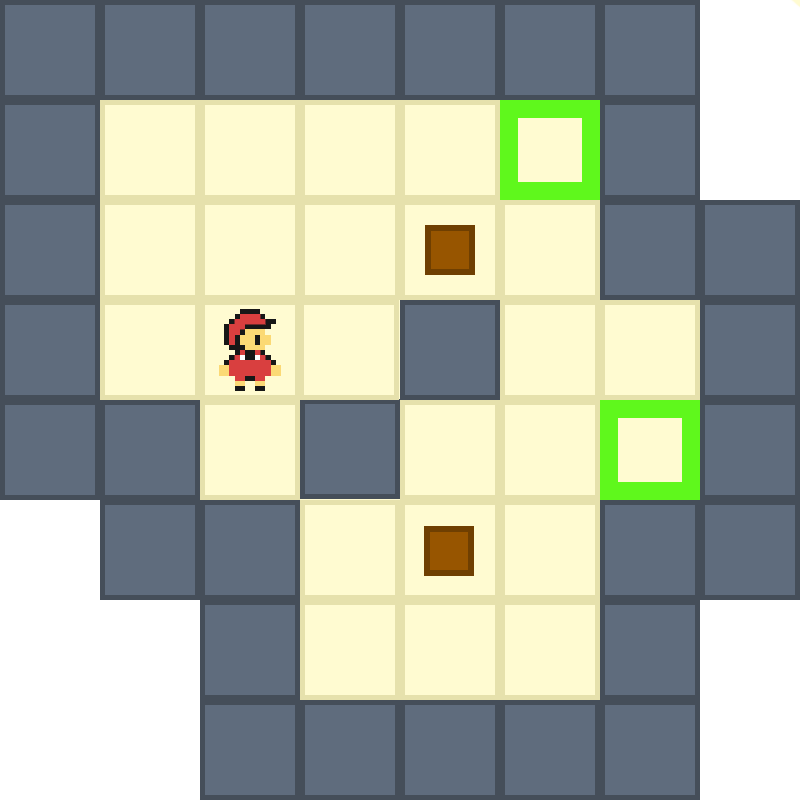
\includegraphics[width=5cm]{sokoban}
    \caption{An example Sokoban level. The grey tiles represent walls, the brown tiles represent boxes, and the green tiles are the targets.}
    \label{fig:sokoban}
\end{figure}

\subsection{Probabilistic model checking}
Model checking is a formal verification technique for analysing and verifying systems. Using model checking tools, one can verify the correctness of certain aspects of the model. For example, a model of a Sokoban level would include the player and box positions, and the solution can be found by querying the state where all boxes are in the solved position.

Probabilistic model checking is a similar technique used to analyse and verify systems that exhibit probabilistic behaviour. A model of a system is often described using a high-level modelling language that defines a set of rules and how these rules modify the state. From this high-level description, the probabilistic model checker will convert it into a probabilistic model by computing the complete set of reachable states. 

The user can supply the model checker with properties, often defined in a property language based on temporal logic. In the case of probabilistic model checking, these are usually quantitative properties, for example, the probability of an event occurring. The model checker calculates these properties by analysing the complete state space generated previously. The full state space analysis yields accurate results, but this comes at the cost of increased computation costs.

PRISM \cite{KNP11}, Storm \cite{Hensel2020}, and Modest \cite{HartmannsH14} are the three probabilistic model checkers chosen to be used in this research, mainly because they have all competed before in QComp.

\subsection{Modelling languages}
The models in this research will be described in both the PRISM language \cite{KNP11} and the JANI specification \cite{Budde2017}. The PRISM language is used throughout the paper because of its simplicity and brevity. 

The PRISM language allows the user to specify variables, which can be bounded, unbounded, and have an initial value:
\begin{lstlisting}[language=PRISM]
x: [0..2];
y: int;
z: bool init false;
\end{lstlisting}
Transitions can be defined and will only be used if a guard on the left-hand side is satisfied:
\begin{lstlisting}[language=PRISM]
[] x=1 & y=2 -> (z'=true);
\end{lstlisting}
The assignments on the right-hand side can be made based on probabilities as well:
\begin{lstlisting}[language=PRISM]
[] x=2 -> 0.5:(z'=false) + 0.5:(z'=true);
\end{lstlisting}
Additionally, ternary statements are also supported and can be used to conditionally assign a value:
\begin{lstlisting}[language=PRISM]
[] y=3 -> (x'=z ? 1 : 2);
\end{lstlisting}

Furthermore, PRISM implements a property specification language that allows the user to proof or analyse certain properties. It can be used to verify quantitive properties such as the minimum or maximum probability of reaching a state:
\begin{lstlisting}[language=PRISM]
Pmin=? [F state]
Pmax=? [F state]
\end{lstlisting}

Time bounds can be introduced into these properties, which can be used to check if a state is reached within $t$ time steps.
\begin{lstlisting}[language=PRISM]
Pmax=? [F<=t state]
\end{lstlisting}

Rewards can be attached to transitions. The expected reward upon reaching a state can also be computed:
\begin{lstlisting}[language=PRISM]
Rmin=? [F state]
Rmax=? [F state]
\end{lstlisting}
The full documentation for the PRISM language and property specification language can be found in the PRISM manual\footnote{PRISM manual - \url{http://www.prismmodelchecker.org/manual/Main/Welcome}}.

\subsection{Sok format}
.sok files\footnote{\url{http://www.sokobano.de/wiki/index.php?title=Sok_format}} are files that contain Sokoban levels. There are currently tens of thousands of user-created levels in this format freely available online. Apart from a few inconsistencies, the format is easy to parse, and the large selection of levels makes it a good choice for this research. The contents of a .sok file are depicted in \autoref{fig:sok}.

\begin{figure}[h]
    \subfloat[\centering ASCII representation of a .sok-file. 'p' represents the player, 'b' represents a box, '.' represents a target location, and '\#' represents a wall.\label{fig:sok_ascii}]{\makebox[0.5\linewidth][c]{\lstinputlisting[basicstyle=\small]{code/level.sok}}}
    \hfill
    \subfloat[\centering Graphical representation of a .sok-file. The brown rectangles represent boxes, the green tiles represent target locations, and the gray tiles represent walls.]{\makebox[0.5\linewidth][c]{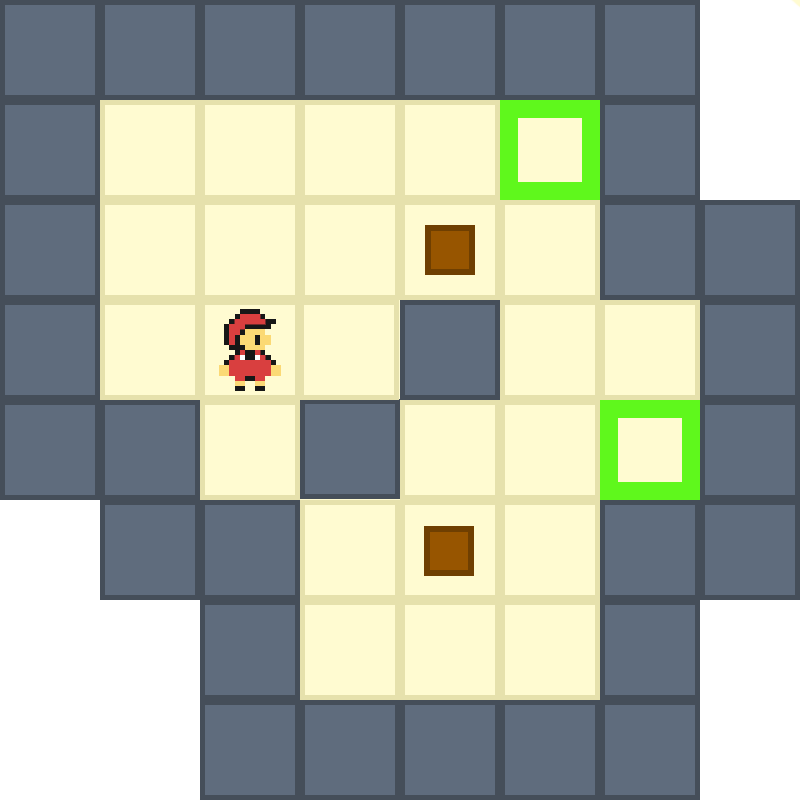
\includegraphics[width=3.0cm,valign=c]{sokoban.png}}}
    \caption{A .sok-file in both its ASCII and graphical representation.}
    \label{fig:sok}
\end{figure}
